\begin{pastexam}[label={px:ccu-114-csb-06}]{中正資工所乙組 114 學年度 第 6 題}
（單選）

(5\%) Given the fully parenthesized arithmetic expression provided below, construct its expression tree and answer the level-order traversal of the tree.
\[ (((((A * B) - (C * D)) - (E / F)) + G) - (H / I)) \]
\begin{enumerate}[label=\Alph*.]
\item \texttt{- + / - G H I - / * * E F A B C D}
\item \texttt{- + - - * A B * / C D E F G / H I}
\item \texttt{- + - - * A B * C D / E F G / H I}
\item \texttt{- + / / G H I - F * E - D * C A B}
\item None of the above
\end{enumerate}
\end{pastexam}

\begin{pastsoln}
答案是 A。

式子已經完全加了括號，每一對括號就是一個運算子節點，最外層的運算子是根（資結書第~7.7~節）：
\begin{center}
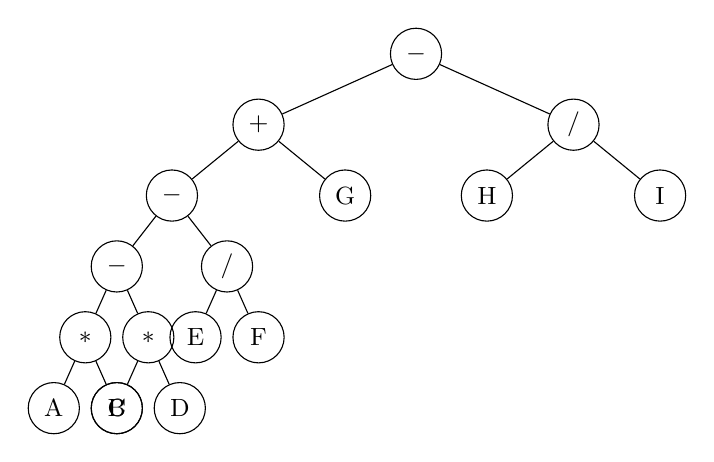
\begin{tikzpicture}[v/.style={circle,draw,minimum size=6.5mm,inner sep=0pt,font=\small},
  level distance=9mm, level 1/.style={sibling distance=40mm}, level 2/.style={sibling distance=22mm},
  level 3/.style={sibling distance=14mm}, level 4/.style={sibling distance=8mm}]
\node[v] {$-$}
  child {node[v] {$+$}
    child {node[v] {$-$}
      child {node[v] {$-$}
        child {node[v] {$*$} child {node[v] {A}} child {node[v] {B}}}
        child {node[v] {$*$} child {node[v] {C}} child {node[v] {D}}}}
      child {node[v] {/} child {node[v] {E}} child {node[v] {F}}}}
    child {node[v] {G}}}
  child {node[v] {/} child {node[v] {H}} child {node[v] {I}}};
\end{tikzpicture}
\end{center}
層序走訪（資結書第~7.3.2~節）一層一層、每層由左往右：
\begin{center}
\begin{tabular}{cl}
\toprule
層 & 節點 \\
\midrule
0 & $-$ \\
1 & $+$\quad / \\
2 & $-$\quad G\quad H\quad I \\
3 & $-$\quad / \\
4 & $*$\quad $*$\quad E\quad F \\
5 & A\quad B\quad C\quad D \\
\bottomrule
\end{tabular}
\end{center}
得 \texttt{- + / - G H I - / * * E F A B C D}，就是 A。

逐項檢查：
\begin{itemize}
\item A：上面的結果。 對。
\item B：\texttt{- + - - * A B \ldots} 第 $1$ 層是 \texttt{+ -}，但根的右子節點是 $H / I$ 的 \texttt{/}；這串比較像前序式的開頭。 錯。
\item C：\texttt{- + - - * A B * C D / E F G / H I} 是這棵樹的\textbf{前序}走訪，不是層序。 錯。
\item D：第 $2$ 層有 \texttt{/ G H I}，但第 $2$ 層的第一個節點是左邊的 \texttt{-}；後半的 \texttt{- F * E - D * C A B} 也不是這棵樹的任何走訪。 錯。
\item E：A 是對的。 錯。
\end{itemize}
\end{pastsoln}
